\newsection{Amazon Web Services}
Amazon Web Services (AWS) is a subsidiary of Amazon that provides on-demand cloud computing platforms to individuals, companies and governments, on a pay-as-you-go basis. These cloud computing web services provide a set of primitive abstract technical infrastructure and distributed computing building blocks and tools. AWS version of virtual computers emulate most of the attributes of a real computer, including hardware central processing units, graphics processing units, memories and storage.

\subsection{Lambda}
AWS Lambda is an Event-Driven serverless computing platform provided by Amazon. It is a computing service that runs code in response to events and automatically manages the computing resources required by that code. The purpose of Lambda is to simplify building applications that are responsive to events and new information. AWS targets starting a Lambda instance within milliseconds of an event.

In this project, lambda functions are the computing core for the execution of all commands and are written in Node.js.

\subsubsection{Write mode Lambda functions}
\begin{figure} [H]
\paragraph{PushOperationAggregateToSQS} \Spazio
Those functions starts the flow and are triggered when fetching the corresponding API gateway URL with a POST request like this: \\
\begin{lstlisting}
	fetch(linkCreateUserAPI_POST, {
		method: 'post',
		headers: {
			'Content-Type': 'application/json',
			'Authorization': 'Bearer ' + localStorage.getItem('id_token')
		},	
		body: JSON.stringify({
			"attribute1": "value1",
			"attribute2": "value2" 
		})
	}).catch(function(error){
			showError(error);
	});
\end{lstlisting}
	\caption{Fetch POST API}\label{}
\end{figure}

\begin{figure} [H]
Once triggered, these functions retrieve the event and put it in the \emph{MessageBody} parameter. The event object doesn't change, it just stringified before sending the message to corresponding SQS queue.

Example:

\begin{lstlisting}
	module.exports.pushCreateUserToSQS = async (event, context, callback) => {
		const utils = require('./utils.js');
		const params = {
			MessageBody: JSON.stringify(event),
			QueueUrl: "https://sqs.eu-central-1.amazonaws.com/582373673306/createUserQueue"
		};
		const res = await utils.pushToSQS(params);
		callback(null, res);
	};
\end{lstlisting}
	\caption{Lambda: pushOperationAggregateToSQS}
\end{figure}

\paragraph{CommandOperationAggregate} \Spazio
These functions validate the values of the attributes before storing the event in the \emph{eventStore} and are triggered when a new event arrives to the corresponding queue. \\ 
If you have to check for duplicated attributes in the database, the function must be marked \emph{async} because it has to wait for the result of the check operation.\\
In this example the function checks for a duplicated userId or email address and if the attributes value is empty, otherwise the event is stored.
\begin{lstlisting}
	module.exports.commandCreateUser = async (event, context, callback) => {
		const utils = require('./utils.js');
		const stringedEvent = event.Records[0].body.toString('utf-8'); 
		const eventParsed = JSON.parse(stringedEvent);
		const stringedBody = JSON.stringify(eventParsed.body);
		const eventToCheck = JSON.parse(stringedBody);
		const checkIdParams = { //params to check for duplicated userId
			TableName: 'user',
			ProjectionExpression: "userId",
			FilterExpression: "userId = :checkId",
			ExpressionAttributeValues: {
				":checkId": eventToCheck.userId
			}
		};
		const userIdAlreadyExists = await utils.asyncCheckScanDB(checkIdParams); 
		if(userIdAlreadyExists)
			callback(null, "userId already exists");
		const checkEmailParams = {  //params to check for duplicated email
			TableName: 'user',
			ProjectionExpression: "email",
			FilterExpression: "email = :checkEmail",
			ExpressionAttributeValues: {
				":checkEmail": eventToCheck.email
			}
		};
		const emailAlreadyExists = await utils.asyncCheckScanDB(checkEmailParams);
		if(emailAlreadyExists)
			callback(null, "Email already exists");
		if(eventToCheck.userId == "" ||eventToCheck.firstName == "" || eventToCheck.lastName == "" || eventToCheck.date == "" || eventToCheck.role == "" || eventToCheck.group == ""){ 
			callback(null, "Empty attributes");
		}
		else{
			utils.storeEvent("user", "executeCreateUserQueue", eventToCheck);
			callback(null, "User event stored");
		}
	};
\end{lstlisting}
\begin{figure}[H]
	\caption{Lambda: commandOperationAggregate}
\end{figure}

\begin{figure} [H]
\paragraph{Mediator} \Spazio
This function catch the \emph{DynamoDB} event and is triggered when a change occurs in a certain table. \\
You have to be careful that the \emph{DynamoDB} events are mapped using the char type attribute value. This is an example: \\

	\centering
	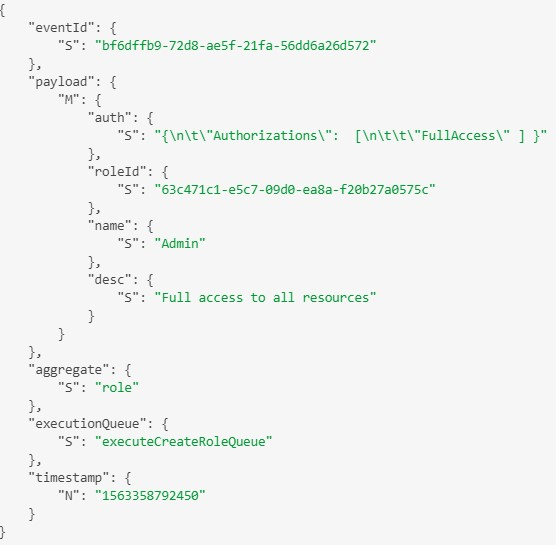
\includegraphics[scale=1]{../Img/dynamoEvent}
	\caption{DynamoDB event object}\label{}
\end{figure}

You can use the \emph{"AWS.DynamoDB.Converter"} module to parse a DynamoDB event object.

\begin{figure} [H]
	\centering
	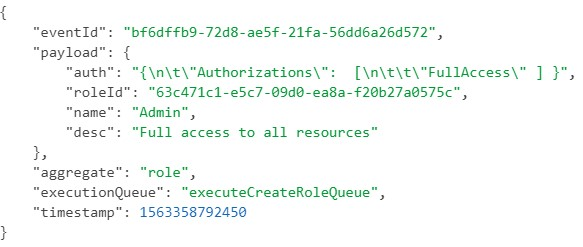
\includegraphics[scale=1]{../Img/parsedDynamoEvent}
	\caption{Parsed DynamoDB event object}\label{}
\end{figure}

\begin{figure} [H]

After that, the mediator retrieves the \emph{executionQueue} parameter from the event object, the payload event is passed with the \emph{MessageBody} and then sends the execution message to corresponding SQS queue. 
\begin{lstlisting}
	module.exports.mediator = (event, context, callback) => { 
		const AWS = require('aws-sdk');
		const SQS = new AWS.SQS();
		const parser = AWS.DynamoDB.Converter; //module to parse dynamodb objects
		try{
			var parsedEvent = parser.unmarshall(event.Records[0].dynamodb.NewImage); 
		}catch (err) {
			console.log(err);
			callback(null, err);
		}
		const params = { //get the SQS params 
			MessageBody: JSON.stringify(parsedEvent.payload),
			QueueUrl: "https://sqs.eu-central-1.amazonaws.com/582373673306/" + parsedEvent.executionQueue
		};
		SQS.sendMessage(params, function(err,data){ //push to SQS
			if(err){
				console.log(err);
				callback(null, err);
			}
			else
				callback(null, "Execution event pushed to SQS");
		});
	};
\end{lstlisting}
	\caption{Lambda: mediator}
\end{figure}


\paragraph{OperationAggregate} \Spazio
These functions execute a single operation using the event payload and are triggered when a new event arrives to corresponding execution queue.\\
Example:
\begin{lstlisting}
	module.exports.createUser = async (event, context, callback) => {
		const AWS = require('aws-sdk');
		const dynamoDb = new AWS.DynamoDB.DocumentClient();
		const stringedBody = event.Records[0].body.toString('utf-8');
		const parsedBody = JSON.parse(stringedBody);
		const params = {
			TableName: 'user',
			Item: parsedBody
		};
		await dynamoDb.put(params, (err, data) => {
			if (err){
				console.log(err);
				callback(null, err);
			}
			else
				callback(null, "User created");
		}).promise();
	};
\end{lstlisting}
\begin{figure} [H]
	\caption{Lambda: operationAggregate}
\end{figure}

\paragraph{Recovery} \Spazio
This function allows you to rebuild the state of the system starting from a given timestamp by replaying all the events which were stored after that time into the \emph{eventStore} table.\\
Is important to re-execute the events one by one and in the correct order(from the oldest one); for this purpose the recovery function implements a sorting algorithm that retrieves an array of events and sorts them by timestamp, and an \emph{async} function which sends every event to the corresponding execution queue.
\begin{lstlisting}
	module.exports.recovery = (event, context, callback) => { 
		const AWS = require('aws-sdk');
		const dynamoDb = new AWS.DynamoDB.DocumentClient();
		const utils = require('./utils.js');
		const queryParams = { 
			TableName: 'eventStore',
			ExpressionAttributeNames:{
			"#eventtimestamp": "timestamp", //timestamp is a reserved keyword
			"#eventaggregate": "aggregate" //aggregate is a reserved keyword 
			},
			ProjectionExpression: "#eventtimestamp, #eventaggregate, payload, executionQueue",
			FilterExpression: "#eventtimestamp >= :timest",
			ExpressionAttributeValues: {
				":timest": parseInt(event.body.timestamp, 10)
			}
		};
		dynamoDb.scan(queryParams, (err, data) => {
			if (err)
				callback(null, err);
			else {
				if(data.Count == 0)
					callback(null, "Events not found");
				else {
					const stringedData = JSON.stringify(data);
					const parsedData = JSON.parse(stringedData);
					var events  = parsedData.Items;
					events.sort((a, b) => { //order events by timestamp from the oldest
					var a1 = a.timestamp, b1 = b.timestamp;
					if (a1 < b1) return -1;
					if (a1 > b1) return 1;
					return 0;
					});
				utils.asyncPushToExecutionQueue(events);
				callback(null, "Recovering...");
				}
			} 
		});
	};
\end{lstlisting}
\begin{figure} [H]
	\caption{Lambda: recovery}
\end{figure}

\subsubsection{Read mode Lambda functions}
\begin{figure} [H]
\paragraph{ReadOperationAggregate} \Spazio
These functions work in the read side of the architecture; they query the database to retrieve the information needed without passing through a SQS queue or a mediator. This kind of events aren't stored into the \emph{eventStore} because they don't change the current system state; these Lambda functions fetch the URL of a GET endpoint using a GET request and listen for a response result.
\begin{lstlisting}
	fetch(linkUserAPI_GET, {
		method: "get",
		headers: {
			'Content-Type': 'application/json',
			'Authorization': 'Bearer ' + localStorage.getItem('id_token')
		}
	}).then(function(response){
			return response;
	}).catch(function(error){
			showError(error);
	});
\end{lstlisting}
	\caption{Fetch GET API}\label{}
\end{figure}

\begin{figure} [H]
Example:
\begin{lstlisting}
	module.exports.readUser = (event, context, callback) => {
		const AWS = require('aws-sdk');
		const dynamoDb = new AWS.DynamoDB.DocumentClient();
		const stringedEvent = JSON.stringify(event);
		const parsedEvent = JSON.parse(stringedEvent);
		const params = { //get user by userId
			TableName: 'user',
			Key: {
				"userId": parsedEvent.userId
			},
			KeyConditionExpression: "userId = :id",
			ExpressionAttributeValues: {
				":id": parsedEvent.userId
			}
		};
		dynamoDb.get(params, (err, data) => {
			const stringedData = JSON.stringify(data);
			if (err)
				callback(null, err);
			else{
				if(data.Count == 0)
					callback(null, "User not found");
				else {
					const response = {
						statusCode: 200,
						headers: {
							'Content-Type': 'application/json',
							'Access-Control-Allow-Origin': '*',
							'Access-Control-Allow-Credentials': true
						},
					body: stringedData
					};
				callback(null, response);
				}      
			}
		});
	};
\end{lstlisting}
	\caption{Lambda: readOperationAggregate}
\end{figure}

\subsubsection{CloudWatch Logs}
Amazon CloudWatch is a monitoring and management service built for developers, system operators, site reliability engineers and IT managers. CloudWatch provides you with data and actionable insights to monitor your applications, understand and respond to system-wide performance changes, optimize resource utilization, and get a unified view of operational health. CloudWatch collects monitoring and operational data in the form of logs, metrics, and events. \\
This tool can be very helpful to debug your Lambda functions and to understand what happens to your system.

\subsection{DynamoDB}
Amazon DynamoDB is a fully managed proprietary NoSQL database service that supports key-value and document data's structures and is offered by Amazon Web Services.
In this project the DynamoDB instance is used for two purpose: it is used to store events and to keep updated the aggregates views.\\
The tables are the following:
\begin{itemize}
	\item \textbf{eventStore}: to keep track of the occurred events;
	\item \textbf{user}: to store users info;
	\item \textbf{role}: to store roles info;
	\item \textbf{authorization}: to store authorizations info;
	\item \textbf{group}: to store groups info.
\end{itemize}

\subsection{API Gateway}
Amazon API Gateway is a fully managed service that makes it easy for developers to create, publish, maintain, monitor, and secure API at any scale. You can create REST and WebSocket API that act as a “front door” for applications to access data, business logic, or functionality from your backend services.

In this project, API endpoints starting the execution flow of a write mode function through a POST request, pushing a new event into the corresponding queue; in fact you have to provide an API endpoint for each function. On the other side, to query the database you have to reach the endpoint through a GET request to get a result response.

\subsection{Authorizer}
A Lambda authorizer (also known as a custom authorizer) is an API Gateway feature that uses a Lambda function to control access to your API.\\
A Lambda authorizer is useful if you want to implement a custom authorization scheme that uses a bearer token authentication strategy or that uses request parameters to determine the caller's identity.\\
When a client makes a request to one of your API's methods, API Gateway calls your Lambda authorizer, which takes the caller's identity as input and returns an IAM policy as output.

There are two types of Lambda authorizers:
\begin{itemize}
	\item A token-based Lambda authorizer (also called TOKEN authorizer) receives the caller's identity in a bearer token, such as a JSON Web Token (JWT);

	\item A request parameter-based Lambda authorizer (also called a REQUEST authorizer) receives the caller's identity in a combination of headers, query string parameters, stage variables and context variables.
\end{itemize}
\begin{figure} [H]
	\centering
	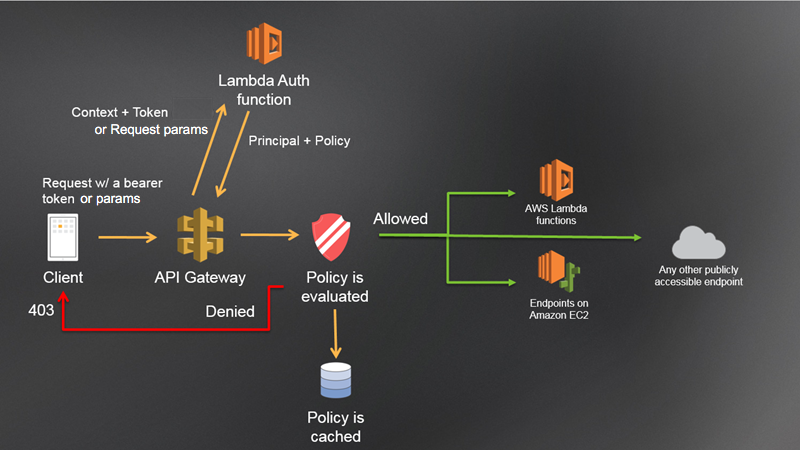
\includegraphics[scale=0.6]{../Img/authorizer}
	\caption{Authorizer workflow}\label{}
\end{figure}

In this project the authorizer is used to protect the access to public endpoints. There are two different authorizer functions, one for admins and one for users. The workflow is the same, the only difference refers to the \emph{client id} and the \emph{public key} provided by \emph{Auht0}, which are needed to authenticate the client identity.

\subsection{Simple Queue Service}
Simple Queue Service(SQS) is a distributed message queuing service introduced by Amazon. It supports programmatic sending of messages via web service applications as a way to communicate over the Internet. SQS is intended to provide a highly scalable hosted message queue that resolves issues arising from the common producer-consumer problem or connectivity between producer and consumer.\\

In this project, for each function you have to use two queues: 
\begin{itemize}
	\item \textbf{OperationAggregateQueue}: this queues receive new events from an API endpoint and trigger the corresponding \emph{commandOperationAggregate} function;
	\item \textbf{ExecuteOperationAggregateQueue}: this queues receive new events from the \emph{mediator} function and trigger the corresponding \emph{operationAggregate} function.
\end{itemize}
